\section{Deployment} \label{sec:deploy}

\begin{figure}[ht!]
    \centering
    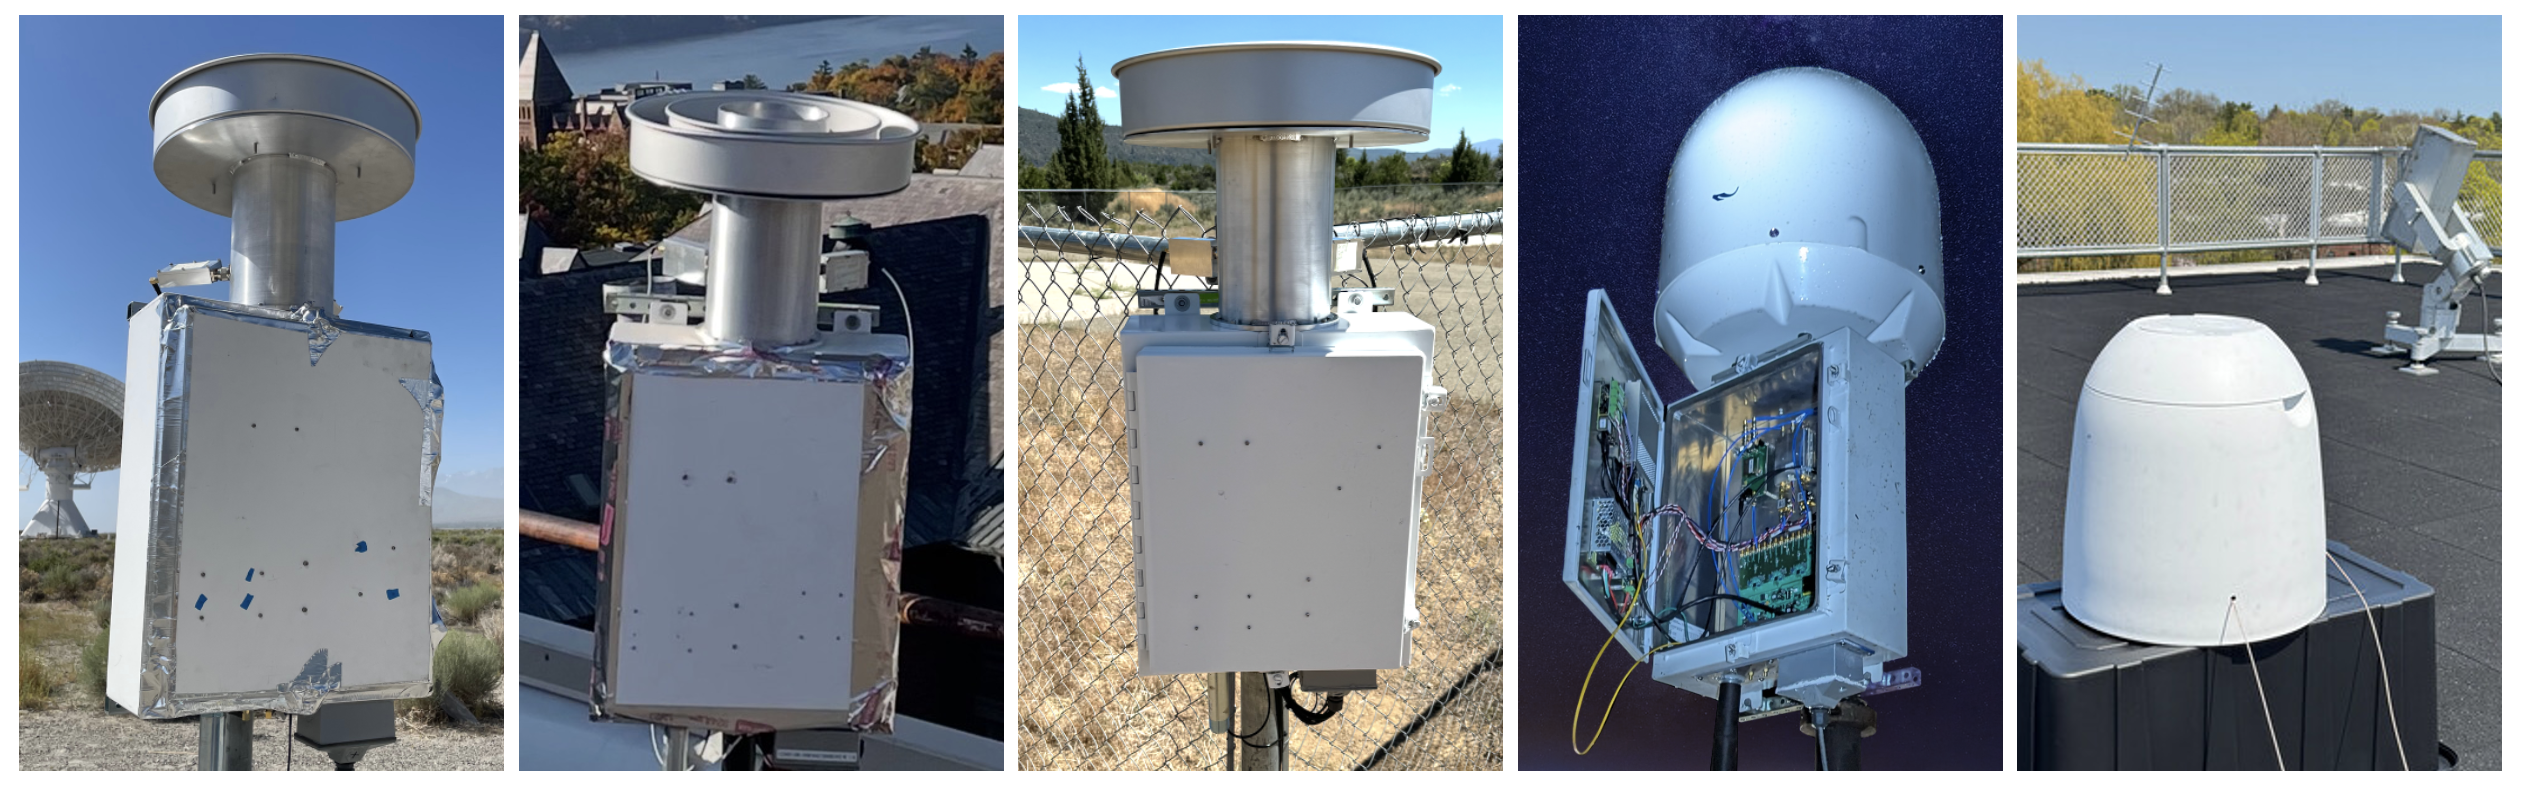
\includegraphics[width=\linewidth]{figures/Terminals.png}
    \caption[Deployed GReX terminals]{Deployed GReX terminals from left to right: Hat Creek Radio Observatory (USA), Cornell University Space Sciences Building (USA), Owens Valley Radio Observatory (USA), and Rosse Observatory (Ireland), and the Smithsonian Astrophysical Observatory at Harvard University (USA).}
    \label{fig:deployments}
\end{figure}

\begin{figure}[ht!]
    \centering
    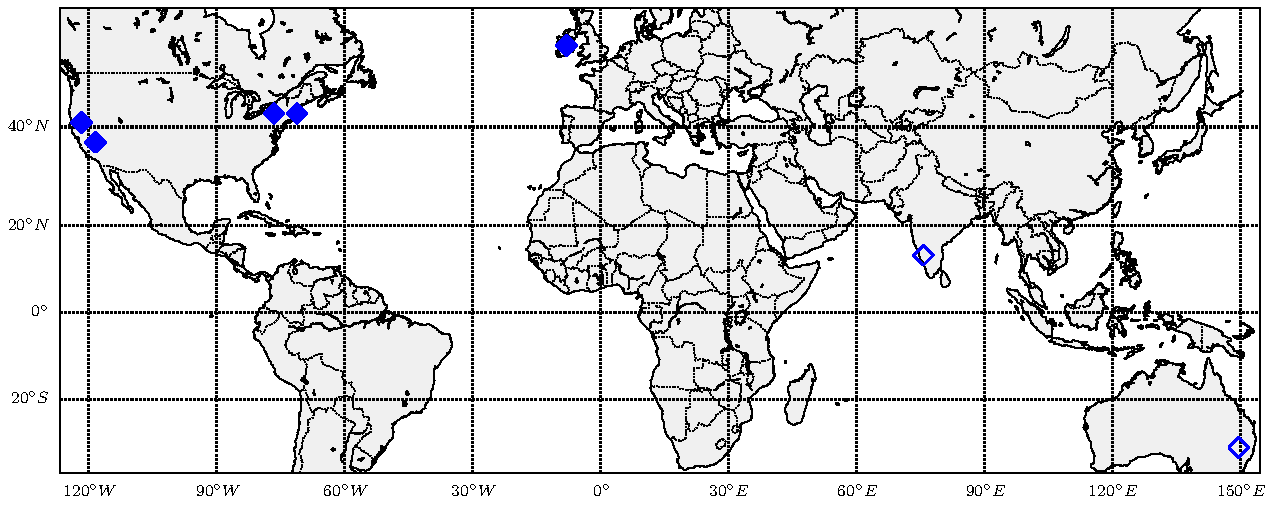
\includegraphics[width=\linewidth]{figures/GReX_Ground_Deployments_Map.pdf}
    \caption[Map of deployed GReX stations]{Mercator map with deployed and on-sky GReX stations ($\blacklozenge$) along with stations at various stages of deployment ($\lozenge$).}
    \label{fig:ground-deployments}
\end{figure}

At the time of writing, five GReX units are currently operating on-sky.
Their locations are shown in \autoref{fig:ground-deployments}, with an additional unit planned for deployment at the Parkes Observatory in New South Wales, Australia.
The first operational unit was deployed at Owens Valley, followed by Cornell, Hat Creek, Birr, and Harvard.
Details of each deployment, including installation processes and site-specific considerations, are outlined below.

\subsection{Owens Valley Radio Observatory}
The initial deployment at the Owen's Valley Radio Observatory took the place of the previous STARE2 system.
We made use of the same location and fiber optic connections.
Installing at the site involved the final assembly of the box, termination of fibers for the Ethernet connection, and testing.
Once the box was powered, we performed Y factor measurements to ensure we achieved our desired sensitivity.

% \begin{figure}[ht!]
%     \centering
%     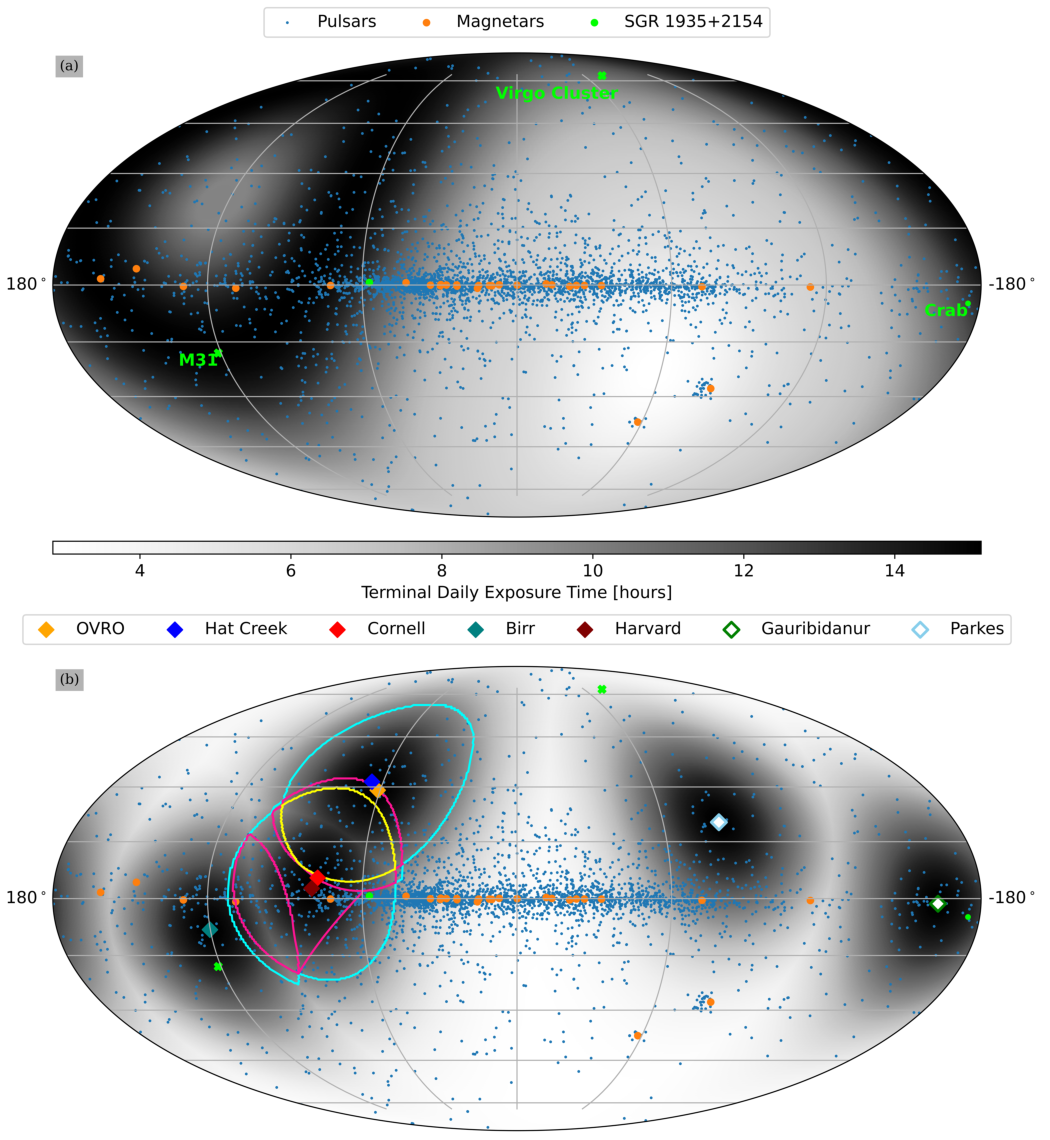
\includegraphics[width=\linewidth]{figures/TerminalSkyMap.pdf}
%     \caption{Figures showing current ($\blacklozenge$) and upcoming ($\lozenge$) GReX terminals (\autoref{fig:ground-deployments}), their coverage of the Galactic plane, and sources of interest. In \textbf{(a)} we show the total exposure time of the GReX system by averaging the simulated 2D Gaussian beam responses of each terminal over a single day. We include markers for the magnetar population taken from the McGill magnetar catelog~\cite{olausenMcGillMagnetarCatalog2014} as that population produced the only detected Galactic FRB. We also include pulsars from the ATNF pulsar catalog~\cite{manchesterAustraliaTelescopeNational2005} as a proxy for the extent of the Galaxy. The Crab is singled out as giant pulses are potentially detectable with GReX. We also include M31 and the Virgo Cluster as locals from which an extraordinarily bright FRB might be detectable by GReX. In \textbf{(b)}, the grayscale heatmap represents a snapshot of the non-overlapping (joint) beam response for all terminals. It is this joint beam response that is averaged over in (a) to avoid overcounting exposure times. The contours enclose regions of sky where multiple beams are greater than their half-maximum value. The cyan, pink, and yellow contours enclose regions with two, three, and four terminals satisfying this condition. Beams are simulated as 2D Gaussians with $\theta_\text{FWHM}=65.18^\circ$, in accordance with our determination of the beam response at $1420.4\,\text{MHz}$ in \autoref{sec:beam_model}.}
%     \label{fig:sky-map}
% \end{figure}

\subsection{Cornell}
The installment of the GReX terminal at Cornell University followed a rough three-stage plan: site testing and preparation, debugging GReX hardware and software, and site installation with first-light measurements.

Prior to receiving any hardware or software, we began a site-searching campaign to identify an optimal site to host the GReX terminal.
This site needs to meet four primary requirements: (1) easy access to electricity and internet, (2) a weatherproof and secure location to host the GReX server, (3) an unimpeded view of the sky from the terminal, and (4) a minimal level of radio frequency interference (RFI) within the observing band.
To facilitate this search, we developed a portable device for recording the RFI environment of a potential site. 
This device includes (i) a chargeable battery-pack for power, (ii) a Siglent Spectrum Analyzer for signal analysis, (iii) and a signal path consisting of a bias-T with 12-V power supply and a 1320-1580 MHz band pass filter\footnote{Mini-Circuits ZX75BP-1450-S+} all of which is contained within a (iv) portable rack case.
For consistency, we used the LNAs and cake pan antenna from the GReX system, with the initial goal of identifying any extreme continuous RFI that would immediately disqualify a potential site.
We then ran follow-up measurements spanning at least one day of collecting time at sites with acceptable RFI levels to search for the presence of any intermittent RFI that was missed during the first survey.
Following this second batch of measurements, we computed Y-factors and equivalent system temperatures (see \autoref{sec:sensitivity} for details) for each of the remaining potential host sites.
All sites showed roughly equivalent baseline system temperatures across the observing band. 
The Space Sciences Building (SSB) roof on Cornell's campus is the lowest system temperature site of those surveyed that meets all four primary site requirements. 
This, combined with the ease of access from having the GReX terminal located in the middle of campus, has led to us selecting the roof of SSB as the permanent Cornell GReX terminal location.

The second stage of deployment is characterized by the arrival of hardware (the server and GReX terminal) on site and subsequent software setup and bug-fixes. 
We received the servers and terminal box at Cornell at the end of June 2023. 
As the second deployed GReX terminal, we spent a few months working closely with team-members at Caltech on hardware and software bug fixes. 
This effort helped develop the comprehensive GReX software guide\footnote{\url{https://grex-telescope.github.io}} for `ground up` installation, from connecting the server to the Raspberry Pi and SNAP board in the terminal box to running the full GReX real-time data capture pipeline. 

With this bug-fixing period complete, we moved to setting up the terminal box on our selected site \autoref{fig:deployments} (Center Left) and taking first-light data collection. 
This included an initial collection of ADC RMS values and observation of the spectra collected on site. 
To prevent overflowing or underflowing of the ADCs, we tuned the adjustable gain in the terminal FEM. 
Two easy astrophysical signals to detect on first light are the presence of the solar continuum (seen as an overall increase in the spectrum as the sun enters the beam) and the HI emission line from Galactic hydrogen centered near $1420.4\,\text{MHz}$. 
The absence of either of these signals indicates that the terminal is not properly observing the sky and requires further fine-tuning, usually either due to an inappropriate FEM gain or spectral leakage within the LNAs. 
Once these checks are passed, we move on to carry out tests of the terminal sensitivity (\autoref{sec:sensitivity}) which will give us estimates of the receiver gain, the system temperature, and the resulting system equivalent flux density (SEFD).

\subsection{Hat Creek Radio Observatory}

The GReX unit deployed at HCRO \autoref{fig:deployments} (Left) was first tested in a screened room using a spectrum analyzer connected to an omnidirectional antenna and external amplifier.
Measurements were conducted with the GReX unit turned off for baseline measurements and then powered on with the box both open and closed with RF absorbers placed inside the enclosure.
Steel wool was added to the fiber cable opening to enhance shielding.
These measurements (discussed in \autoref{sec:self_rfi}) show that the self-generated RFI is stronger than expected, and necessitated installation at a more remote location on site to avoid interference with other experiments.

\subsection{Rosse Observatory}
The deployment of the GReX unit in Ireland was completed in December 2024 at the radio observatory of Trinity College Dublin.
The Rosse Observatory is situated in Birr, in the relatively low population density Irish Midlands.
The site already hosts the Irish LOw Frequency Array (LOFAR) station~\cite{vanhaarlemLOFARLOwFrequencyARray2013,murphyFirstResultsREALtime2021} and other smaller experiments.
As the GReX deployment was in close proximity to the LOFAR station, any unintended emission from the GReX unit in the LOFAR band was measured in lab, prior to deployment, see \autoref{sec:self_rfi}.
Due to the harsher weather conditions in Ireland, the GReX unit underwent further waterproofing with extra sealant on the box where all components are housed (see \autoref{fig:box_inside}).
The most notable modification is the use of a radome housing, as it is radio transparent and often used on marine vessels to protect equipment from harsh outdoor elements \autoref{fig:deployments} (Right).


\subsection{Self-Generated RFI} \label{sec:self_rfi}

\begin{figure}[ht!]
    \centering
    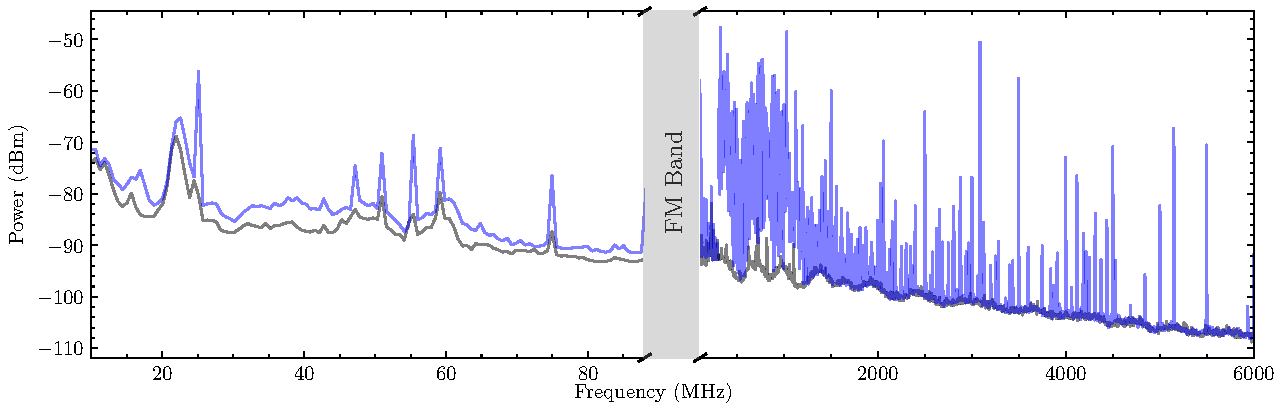
\includegraphics[width=\linewidth]{figures/GReX_Ground_Deployments_withFoV.pdf}
    \caption[GReX EMI spectrum]{Measured power spectrum from $10-6000\,\text{MHz}$ of GReX electromagnetic interference (EMI). The blue trace shows the spectrum when the GReX box is powered on and positioned nearby, while the gray trace represents the baseline measurement taken with the spectrum analyzer. The frequency ranges $10-300\,\text{MHz}$ and $300-6000\,\text{MHz}$ were measured independently by the Birr and Hat Creek teams, respectively.}
    \label{fig:RFISpectrum}
\end{figure}

\begin{figure}[ht!]
    \centering
    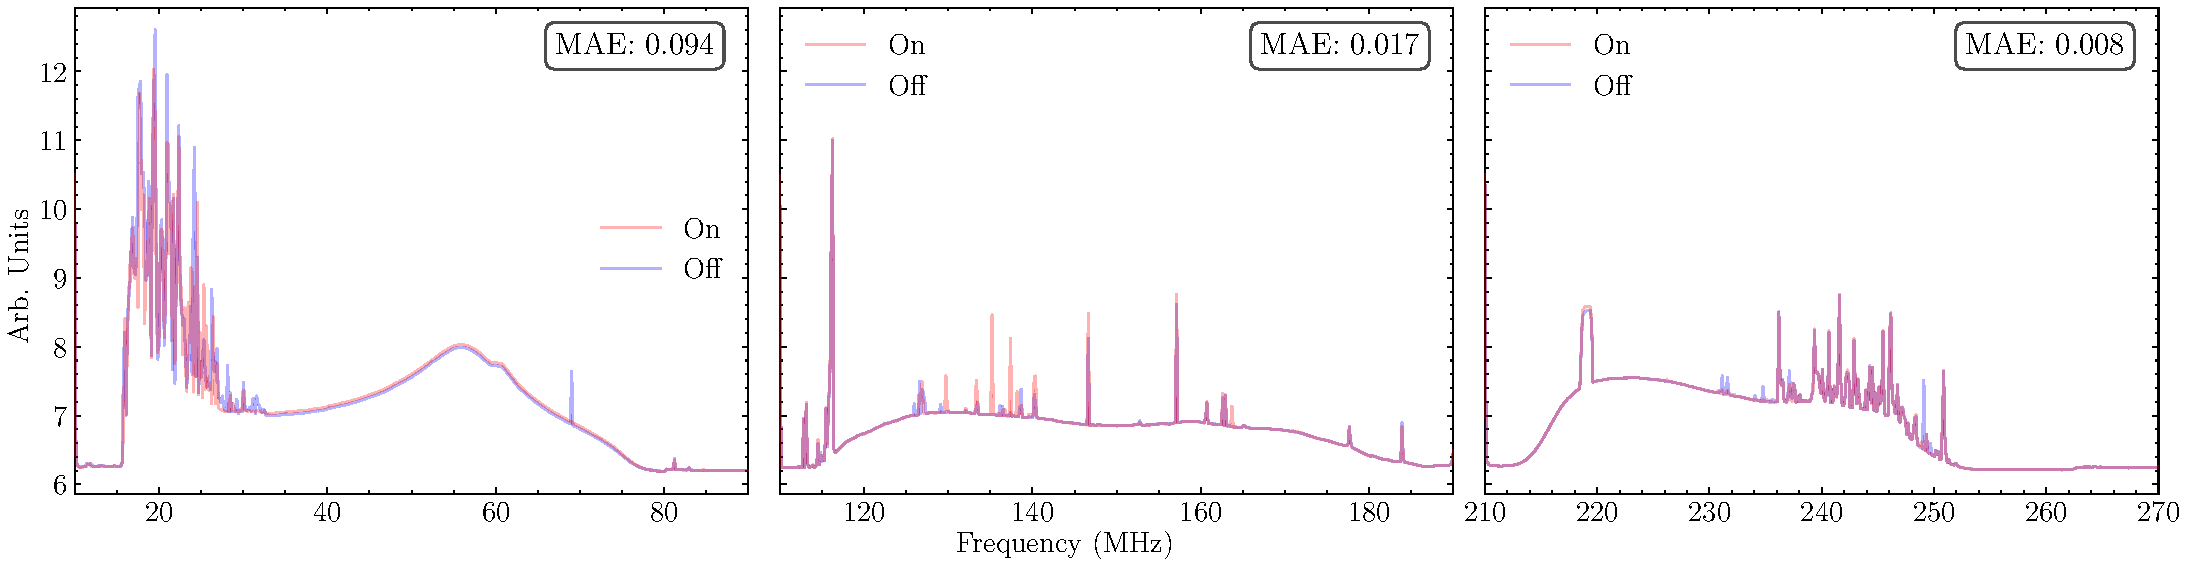
\includegraphics[width=\linewidth]{figures/sst_test.pdf}
    \caption[I-LOFAR GReX EMI Test]{15-minute Stokes I spectra measured using I-LOFAR with the GReX unit powered on and off, covering all observing modes from $10-270\,\text{MHz}$. The mean absolute error (MAE) was calculated for each measurement, comparing the powered-on spectrum to the baseline (powered-off) measurement.}
    \label{fig:IE613-sst-test}
\end{figure}

As GReX is intended to be hosted at radio observatories as well as universities, tests of the self-generated RFI are critical to maintain spectrum purity at sensitive sites.
Tests were performed in screened rooms at both HCRO and CSIRO.
Additionally, Stokes I data were taken using I-LOFAR at Birr while GReX was operational.
Both of the results from HCRO and CSIRO indicate that GReX in its current form is not yet suitable for installation close to sensitive telescopes such as the Parkes 64m.
The emission for a closed box in a screened room is shown in \autoref{fig:RFISpectrum}.
We believe the RFI retrofitting of the commercial enclosure used to house the electronics is primarily at fault.
Further experiments with other RFI gaskets and conductive tape show a marked improvement in radiated power, but not totally acceptable for sensitive sites, especially at L-band.
However, Stokes I data from I-LOFAR (shown in \autoref{fig:IE613-sst-test}) show no appreciable contamination.
Additionally, the various experiments at OVRO such as the DSA-110 and LWA have also not noticed any increase in local RFI.

While some mitigations have substantially improved the unit's EMI profile, the box remains a moderate RFI source.
The self-generated RFI has not proven to be an issue for the FRB detection pipeline, nor has it interfered with experiments at operational radio observatories.
However, the emission remains an open issue and prevents installation at some sites.
Further work is needed to identify problematic components and improve shielding.
